%package list
\documentclass[titlepage,twocolumn]{article}
\usepackage{cite}
\usepackage[utf8]{inputenc}
\usepackage{float}
\usepackage{graphicx}
\usepackage{multirow}
\usepackage{amsmath}
\usepackage{caption}
\usepackage[portuguese]{babel}
\usepackage[top=1cm,bottom=1.5cm,left=1cm,right=1cm]{geometry}
\renewcommand{\figurename}{Figura}
\renewcommand{\tablename}{Tabela} 
\title{TR1: Projeto 2 - Simulação da Camada Física}


%Authors List

\author
{Amélia Oliveira Freitas da Silva\\
Departamento de Ciência da Computação - CIC\\
Universidade de Brasília\\
Brasília, DF\\
Email: 190037971@aluno.unb.br
}

\begin{document}
\begin{titlepage}
    \maketitle
\end{titlepage}

\section{Introdução}

A camada física é a responsável pela transmissão de bits (ou grupos de bits) entre agentes, permitindo a implementação de protocolos de camadas superiores.

São sua responsabilidade as seguintes operações:

\begin{itemize}
    \item Conversão de um conjunto de informações em uma se\-quên\-cia interpretável de pulsos com ou sem um \textit{clock}, a \textbf{Codificação}.
    \item Conversão dos pulsos digitais em sinais fisicamente transportáveis (geralmente analógicos); o que no caso de ondas portadoras, é a \textbf{Modulação}.
    \item O transporte físico do sinal entre os a\-gen\-tes.
    \item Conversão do sinal físico de volta aos pulsos digitais; o que no caso de ondas portadoras, é a \textbf{Demodulação}.
    \item Conversão dos pulsos digitais de volta à informação original, a \textbf{Decodificação}.
\end{itemize}

O objetivo da simulação é implementar a transmissão simples de bits entre agentes, que usarão a conexão para uma camada de aplicação simples (envio e mostra de bytes em ASCII).

\subsection{Modulação/Demodulação}
\label{sec:modemod}
Geralmente a transmissão de sinais é realizada utilizando uma quantidade analógica variando em ondas, como uma variação de intensidade de corrente/potencial elétrico, ondas eletromagnéticas (rádio, transmissões óticas) ou outras variantes.

À onda que leva o sinal damos o nome de \textbf{Onda Portadora}. Esta onda é geralmente definida por uma senóide e possui os seguintes parâmetros:
\[ O_{portadora}(t) = \alpha sin(t\omega+\theta) \]
\begin{itemize}
    \item $\alpha$: Amplitude da onda. Metade da distância entre o pico e o vale.
    \item $\omega$: Velocidade angular/frequência da onda. Inverso do período, que é o tempo necessário para um ciclo completo da onda.
    \item $\theta$: Fase. Deslocamento da onda no tempo. Uma fase positiva desloca a onda à esquerda.
\end{itemize}

\begin{figure}[H]
    \begin{center}
        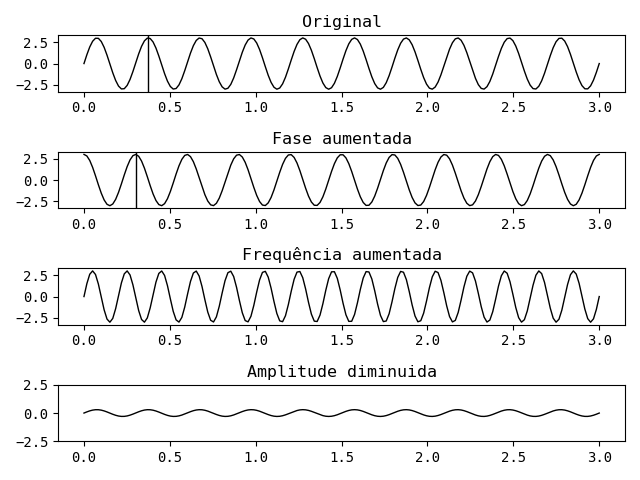
\includegraphics[width=9.5cm]{imgs/onda_portadora.png}
        \caption{Ilustração dos parâmetros de onda}
        \label{fig:onda}
    \end{center}
\end{figure}

Alterando um ou mais dos três parâmetros no emissor podemos transmitir informações ao receptor. Essa alteração é denominada \textbf{Modulação} (como nos rádios AM - \textit{Amplitude Modulation} - e FM - \textit{Frequency Modulation}).

Trabalharemos com a modulação da fase para a nossa si\-mulação. A modulação de fase é comumente utilizada para transmissões digitais em ambientes com pouco ruido por sua resistência moderada a ruídos e boa eficiência espectral.

A modulação é executada simplesmente pela alteração do parâmetro na onda portadora, enquanto a demodulação de um sinal modulado em fase é baseada na multiplicação por um sinal de referência.

\begin{equation}
    \label{eq:multi}
        sin(\omega t+\theta_1)sin(\omega t+\theta_2) = \frac{1}{2}[cos(\theta_1-\theta_2) - cos(2\omega t+(\theta_1+\theta_2))]
\end{equation}

\begin{figure}[H]
    \begin{center}
        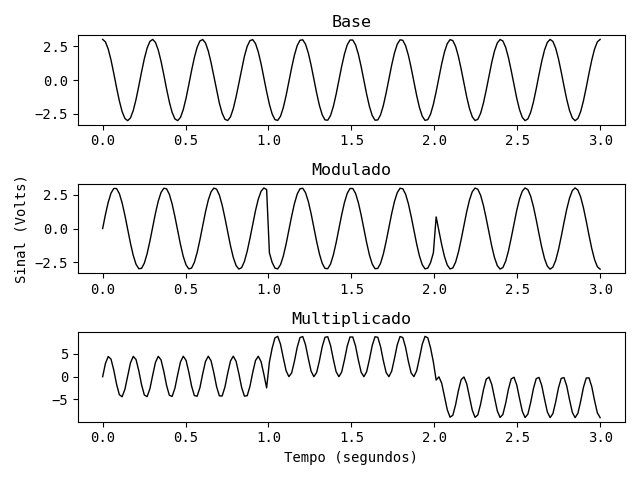
\includegraphics[width=9.5cm]{imgs/modulacao_fase.png}
        \caption{Ilustração da  multiplicação de senoides}
        \label{fig:demod}
    \end{center}
\end{figure}

Pode-se ver que a onda resultante possui um deslocamento de $\frac{cos(\theta_1-\theta_2)}{2}$ em relação ao zero. Isso nos permite identificar a diferença entre a fase do sinal e a fase de referência, ou seja, a informação por ela transmitida.

Geralmente são usadas duas fases na modulação: 0 e $\frac{\pi}{2}rad$. Na figura \ref{fig:demod} (seção \ref{sec:modemod}) podemos ver exemplos com modulação de $\frac{\pi}{2}$, 0 e $-\frac{\pi}{2}$, além do resultado da multiplicação dos sinais, ilustrando o deslocamento causado pela modulação.

Aplicando-se uma média móvel exponencial ao produto dos sinais, a distinção entre os três estados fica ainda melhor definida.

\begin{figure}[H]
    \begin{center}
        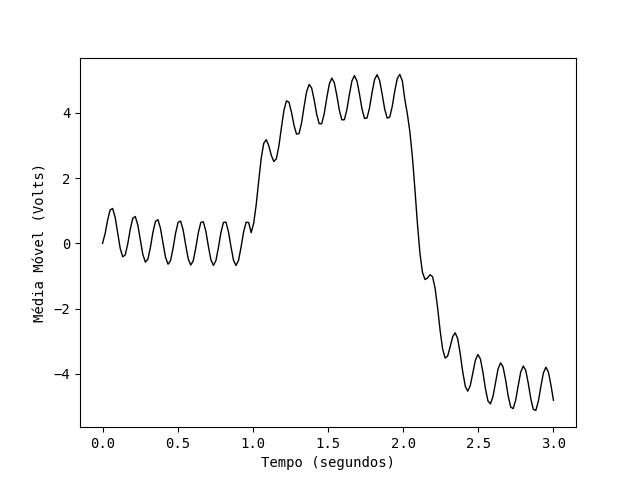
\includegraphics[width=9.5cm]{imgs/mediamovel_modulacao_fase.png}
        \caption{Média móvel exponencial do produto dos sinais}
        \label{fig:medmov}
    \end{center}
\end{figure}

\subsection{Codificação/Decodificação}

Estabelecidos meios para a transmissão de pulsos e estados definidos, resta definir como a informação que transmitiremos será comunicada por meio desses estados e pulsos.

\subsubsection{Codificação Binária}
\label{sec:binaria}

\begin{figure}[H]
    \begin{center}
        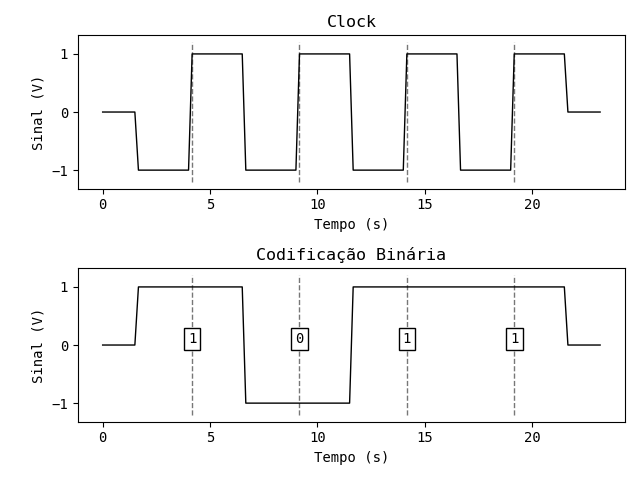
\includegraphics[width=9.5cm]{imgs/codificacao_bnaria.png}
        \caption{Demonstração da codificação binária}
        \label{fig:binaria}
    \end{center}
\end{figure}

Na codificação binária, a representação dos bits é diretamente análoga à sequência de pulsos transmitidos.

São definidos dois valores de referência para o sinal/tensão (\texttt{ALTA}, \texttt{BAIXA}). A cada subida do \textit{clock}, lemos o valor atual do sinal. Tensões na referência alta são geralmente lidas como "1"s e tensões na referência baixa são lidas como "0"s.

Como são usadas duas referências com valores geralmente não-nulos, a forma mais comum dessa codificação é conhecida como \textit{NRZ} (\textit{No Return to Zero}), dado que o sinal nunca retorna a um estado "indefinido/intermediário", permanecendo sempre em um que carrega informação.

Embora simples, essa codificação possui problemas ao representar longas cadeias de "1"s ou "0"s, pois não há transições entre as tensões altas e baixas nesses casos. Considere a figura anterior (Figura \ref{fig:binaria}, \ref{sec:binaria}): sem a referência do \textit{clock}, não poderíamos saber exatamente quantos "1"s foram transmitidos entre \textit{t=12.5s} e \textit{t=22.5s}.

\subsubsection{Codificação Manchester}
\label{sec:manchester}
\begin{figure}[H]
    \begin{center}
        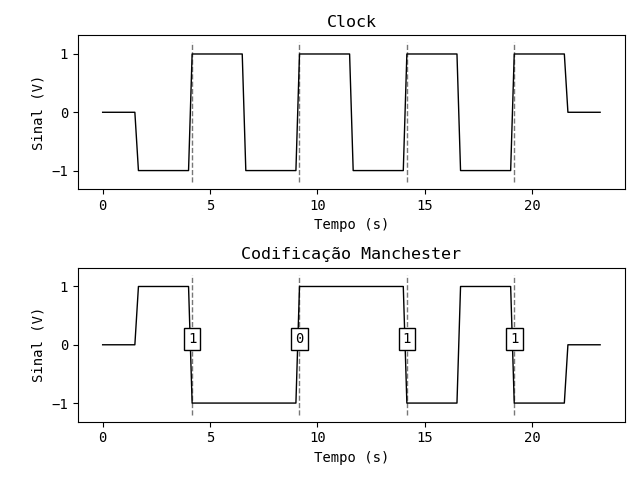
\includegraphics[width=9.5cm]{imgs/codificacao_manchester.png}
        \caption{Demonstração da codificação Manchester}
        \label{fig:manchester}
    \end{center}
\end{figure}

A codificação Manchester resolve o problema da falta de transições em cadeias contíguas representando "0"s e "1"s não como estados definidos, mas como transições a cada sinal de \textit{clock}. No exemplo acima, tran\-sições "\texttt{ALTO} $\rightarrow$ \texttt{BAIXO}"\   representam "1"s e transições "\texttt{BAIXO} $\rightarrow$ \texttt{ALTO}", "0"s. Há transições fora do sinal de \textit{clock} quando há bits repetidos contíguos.

A presença de transições sempre que há um sinal de \textit{clock} permite que ajustemos a nossa referência de tempo de maneira independente. Conhecedo aproximadamente o intervalo de cada bit (período do \textit{clock}), podemos inclusive decodificar o sinal sem a necessidade de temporização, o que torna o sinal \textit{auto-temporizante} (\textit{self-clocking}).

A codificação Manchester pode ser obtida como o resultado do operador binário "Ou exclusivo"\ entre o sinal do \textit{clock} e a representação binária.
\[
    S_{manchester} = S_{binario} \otimes S_{clock}
\]

\subsubsection{Codificação Bipolar}
\label{sub:bipolar}

\begin{figure}[H]
    \begin{center}
        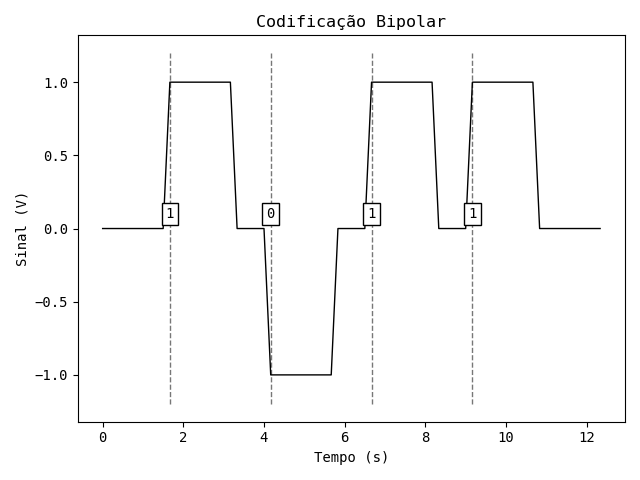
\includegraphics[width=9.5cm]{imgs/codificacao_bipolar.png}
        \caption{Demonstração da codificação Bipolar}
        \label{fig:bipolar}
    \end{center}
\end{figure}

Na codificação bipolar, ao contrário das anteriores, não necessitamos de um \textit{clock} em ponto algum, seja na geração ou decodificação do sinal. Realizamo-no pelo uso de três valores de referência (\texttt{ALTO},\texttt{NEUTRO},\texttt{BAIXO}), o que a torna uma codificação \textit{pseudoternária}.

O valor \texttt{NEUTRO} é utilizado como um separador entre os bits transmitidos. Transições "\texttt{NEUTRO}$\rightarrow$\texttt{ALTO}" indicam "1"s, transições "\texttt{NEUTRO}$\rightarrow$\texttt{BAIXO}" indicam "0"s (ou vice-versa a depender da especificação).

A existência de um separador de bits dispensa o uso de um \textit{clock} externo, visto que cada transição já possui toda a informação necessária para a decodificação. Essa facilidade vem a custo da precisão necessária para a demodulação do sinal, pois precisa-se distinguir três níveis dentro do mesmo espaço de fase/amplitude/frequência, aumentando a sensibilidade do sistema a ruídos.

\section{Implementação}

A premissa adotada para a implementação da simulação foi definida pelos seguintes pontos:

\begin{itemize}
    \item A simulação deve possuir parâmetros diretamente análogos a parâmetros físicos (isto é, a simulação deve ser reprodutível por um sistema físico).
    \item Os sistemas são causais e dinâmicos, recebendo a cada "quadro" da simulação apenas os parâmetros atuais e dependendo apenas deles (e, implicitamente, das entradas em tempos anteriores).
\end{itemize}

\subsection{Modulação/Demodulação}

A função \texttt{onda\_base} gera o valor de uma onda portadora de amplitude 1 para um certo ponto no tempo, dados os parâmetros de frequência (implicitamente, pelo período), e fase.

As classes de modulação e demodulação possuem três estados possíveis: \texttt{enum estado = }\{\texttt{BAIXO,NEUTRO,ALTO}\}. A cada intervalo de tempo, elas atualizam seus parâmetros de acordo com a especificação seguinte e disparam os eventos respectivos.

\subsubsection{Classe Modulador}

A classe modulador tem uma saída analógica (\texttt{double saida}), gerada a cada intervalo de tempo baseada em seu estado atual (\texttt{estado S}), que define a fase e parâmetros de frequência, amplitude, etc.

\begin{center}
    \begin{tabular}{c | c }
        \hline
        Estado & Fase\\
        \hline
        \texttt{BAIXO} & $\frac{\pi}{2}$\\
        \texttt{NEUTRO} & 0\\
        \texttt{ALTO} & $-\frac{\pi}{2}$\\
        \hline
    \end{tabular}
    \captionof{table}{Referências de fase para diferentes estados}
    \label{tab:fasestados}
\end{center}

Um intervalo de tempo é marcado pela chamada da função \texttt{Modulador::passatempo}.

O sistema é análogo à implementação física de um seletor com três saídas definidas por geradores de onda com as fases listadas e a seleção definida pelo estado atual.

\subsubsection{Classe Demodulador}

A classe demodulador tem uma saída discreta (\texttt{estado S}) e dispara eventos a cada mudança de estado, descrevendo transições positivas e negativas (listadas abaixo). Como entrada, ela recebe a amostra atual do sinal (saída de um modulador, atrasada ou não).

\begin{center}
    \begin{tabular}{c | c }
        \hline
        Estados & Evento\\
        \hline
        \texttt{BAIXO}$\rightarrow$\texttt{NEUTRO} & \texttt{Demodulador::posedge}\\
        \texttt{NEUTRO}$\rightarrow$\texttt{ALTO} & \texttt{Demodulador::posedge}\\
        \texttt{ALTO}$\rightarrow$\texttt{NEUTRO} & \texttt{Demodulador::negedge}\\
        \texttt{NEUTRO}$\rightarrow$\texttt{BAIXO} & \texttt{Demodulador::negedge}\\
        \hline
    \end{tabular}\\

    \small{*Transições diretas entre \texttt{ALTO} e \texttt{BAIXO} nunca acontecem sem a passagem por um estado \texttt{NEUTRO}}
    \captionof{table}{Eventos de transição de estado}
\end{center}

O demodulador possui sua própria onda de referência, calculada com uma fase de referência \texttt{Demodulador::fase}.

A cada intervalo de tempo, o demodulador multiplica o sinal atual pelo sinal de referência (vide figura \ref{fig:demod}, seção \ref{sec:modemod}), adiciona o resultado a uma média móvel exponencial (figura \ref{fig:medmov}, mesma seção) e toma um dos seguintes caminhos:
\begin{itemize}
    \item Modo \textbf{Ajuste} (função \texttt{Demodulador::ajusta\_fase}): o demodulador compara o valor atual da média móvel a uma referência de valor \texttt{ALTO} e, assumindo que a entrada está em um estado \texttt{ALTO}, ajusta a fase para que a média se aproxime da referência (ou seja, alinhando os picos das ondas).
    \item Modo \textbf{Ativo} (função \texttt{Demodulador::recebe\_amostra}): o demodulador compara o valor atual da média móvel à referência do estado atual. Caso a distância absoluta seja maior que \texttt{Demodulador::delta\_max}, uma mudança de estado ocorre, alterando \texttt{Demodulador::S} e causando um dos eventos listados acima.
\end{itemize}

O modo de ajuste de fase é importante para compensar diferenças de fase entre o modulador e demodulador, que podem acontecer por falta de sincronização natural entre os parâmetros em situações reais, ou até mesmo pela distância e consequente atraso de transporte da onda entre os dois (como demonstrável na simulação).

A operação de multiplicação de sinais possui um componente físico que realiza a mesma operação, enquanto a média móvel exponencial é equivalente à implementação de um circuito RC (com a entrada passando a um capacitor por meio de um resistor e a saída sendo a diferença de potencial entre os polos do capacitor).

A taxa de alisamento $\sigma$ é relacionada à capacitância $C$ e a resistência $R$ do circuito da seguinte forma:
\begin{equation}
    RC = \Delta_T \left(\frac{1-\sigma}{\sigma}\right)
\end{equation}

\subsection{Codificação/Decodificação}

As classes \texttt{Transmissor}(codificador) e \texttt{Receptor}(decodificador) possuem, respectivamente, dois moduladores e demoduladores representando os sinais de clock e dados. Neste nível, abstraimos a parte de modulação e focamos apenas nas transições de estados lógicos.

\subsubsection{Classe Transmissor(Codificador)}

O transmissor possui um \textit{buffer} de bytes a serem transmitidos (um detalhe para facilitar a implementação da camada de aplicação, baseada em bytes, ainda que a transmissão seja bit-a-bit). Uma consequência dessa estrutura é que o transmissor só para a codificação após transmitir múltiplos de 8 bits, mas os bits não utilizados podem ser simplesmente ignorados.

Para cada bit a transmitir, o codificador passa por um ciclo definido, alterando o estado dos seus moduladores para transmitir a informação codificada. Para a codificação Manchester, foi introduzido um pequeno atraso no sinal de dados para facilitar a futura decodificação.

\begin{figure}[H]
    \begin{center}
        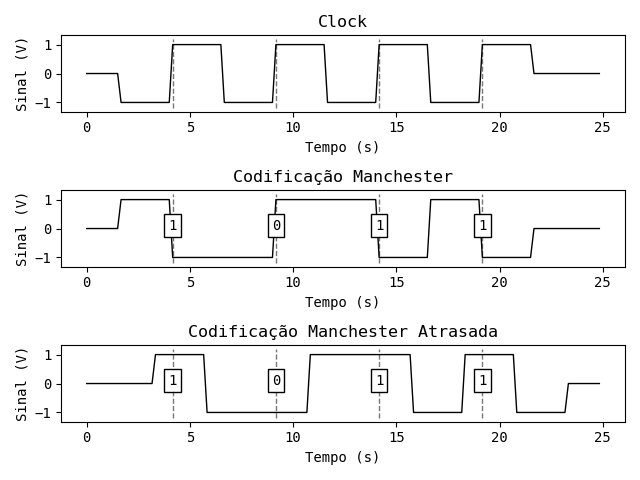
\includegraphics[width=9.5cm]{imgs/codificacao_manchester_atrasada.png}
        \caption{Codificação Manchester com atraso}
        \label{fig:manchestera}
    \end{center}
\end{figure}

Os ciclos de transmissão para cada codificação são os se\-guintes:

\begin{itemize}
    \item \textbf{Codificação binária}:
    \begin{itemize}
        \item Tempo 0: O modulador de dados vai para o estado $Bit_{atual}$;
        \item Tempo 1: O modulador de clock vai para o estado \texttt{ALTO};
        \item Tempo 2: O modulador de clock vai para o estado \texttt{BAIXO}.
    \end{itemize}
    \item \textbf{Codificação Manchester}:
    \begin{itemize}
        \item Tempo 0: O modulador de clock vai para o estado \texttt{BAIXO}
        \item Tempo 1: O modulador de dados vai para o estado $Bit_{atual}$;
        \item Tempo 2: O modulador de clock vai para o estado \texttt{ALTO};
        \item Tempo 3: O modulador de dados vai para o estado $\overline{Bit_{atual}}$  (equivalente a \textit{clock} $\otimes$ bit atual);
    \end{itemize}
    \item \textbf{Codificação bipolar}:
    \begin{itemize}
        \item Tempo 0: O modulador de dados vai para o estado $Bit_{atual}$;
        \item Tempo 1: O modulador de dados vai para o estado \texttt{NEUTRO};
    \end{itemize}
\end{itemize}

No código, os ciclos estão divididos em quatro passos nos três casos, com passos redundantes nos ciclos com menos de quatro.

O trânsito entre todos os passos do transmissor leva um tempo fixo e ao final de cada ciclo garantimos a codificação de um bit. A taxa de transmissão de bits é, pois, o inverso do tempo de um bit (\texttt{Transmissor::periodo\_bit}).

\subsubsection{Classe Receptor (Decodificador)}

O receptor lê e interpreta os eventos dos demoduladores de maneira diferente a depender da codificação utilizada. Um \textit{buffer} de 8 bits é utilizado para facilitar a comunicação com a aplicação, causando um evento (\texttt{Receptor::on\_char}) quando os 8 bits são preenchidos.

Para cada codificação, os eventos são interpretados de acordo com as definições a seguir:

\begin{center}
    \begin{tabular}{|c | c |}
        \hline
        Estado (Clock) & Ação Binária\\
        \hline
        \texttt{BAIXO}$\rightarrow$\texttt{NEUTRO} & N/A\\
        \texttt{NEUTRO}$\rightarrow$\texttt{ALTO} & Atribui o valor atual do sinal ao bit\\
        \texttt{ALTO}$\rightarrow$\texttt{NEUTRO} & N/A\\
        \texttt{NEUTRO}$\rightarrow$\texttt{BAIXO} & N/A\\
        \hline
    \end{tabular}\\
    \captionof{table}{Transições para a codificação binária}
\end{center}

\begin{center}
    \begin{tabular}{|c | c |}
        \hline
        Estado (Clock) & Ação Manchester\\
        \hline
        \texttt{BAIXO}$\rightarrow$\texttt{NEUTRO} & N/A\\
        \texttt{NEUTRO}$\rightarrow$\texttt{ALTO} & Atribui o valor atual do sinal ao bit\\
        \texttt{ALTO}$\rightarrow$\texttt{NEUTRO} & N/A\\
        \texttt{NEUTRO}$\rightarrow$\texttt{BAIXO} & N/A\\
        \hline
    \end{tabular}\\
    \captionof{table}{Transições para a codificação Manchester (Atrasada)}
\end{center}

\begin{center}
    \begin{tabular}{|c | c |}
        \hline
        Estado (Dado) & Ação Bipolar\\
        \hline
        \texttt{BAIXO}$\rightarrow$\texttt{NEUTRO} & N/A\\
        \texttt{NEUTRO}$\rightarrow$\texttt{ALTO} & $Bit_{atual} = 1$\\
        \texttt{ALTO}$\rightarrow$\texttt{NEUTRO} & N/A\\
        \texttt{NEUTRO}$\rightarrow$\texttt{BAIXO} & $Bit_{atual} = 0$\\
        \hline
    \end{tabular}\\
    \captionof{table}{Transições para a codificação Bipolar}
\end{center}

Como atrasamos a codificação manchester, na transição do clock para o estado \texttt{ALTO}, o valor do sinal ainda não foi atualizado de
\[Bit_{transmitido} \oplus 0 = Bit_{transmitido}\] para
\[Bit_{transmitido} \oplus 1 = \overline{Bit_{transmitido}}\]
(O que aconteceria no próximo passo do ciclo de transmissão)

Podemos então simplesmente lê-lo diretamente, como na binária, simplificando bastante a decodificação.

A cada definição de bit, passamos para o próximo até preencher os 8, voltando ao primeiro depois do disparo do evento.

\subsection{Aplicação}

Na camada de aplicação, abstraimos a codifica\-ção/de\-codificação dos bits (e empacotamento em bytes), então trabalharemos somente com a interface do usuário e em dar significados aos bytes transmitidos.

A aplicação é baseada na transmissão de letras no padrão ASCII de um agente a outro por meio do sistema até agora descrito. Cada tecla digitada é enviada como um byte ao transmissor, decodificada no receptor e adicionada a um \textit{buffer} para visualização.

Algumas teclas possuem funções especiais e não serão transmitidas, mas sim causarão eventos específicos ao serem pressionadas:

\begin{center}
    \begin{tabular}{|c | c |}
        \hline
        Tecla & Efeito\\
        \hline
        \texttt{1} & Usa a codificação binária\\
        \texttt{2} & Usa a codificação Manchester\\
        \texttt{3} & Usa a codificação bipolar\\
        \texttt{ESPAÇO} & Redefine a simulação\\
        \hline
    \end{tabular}\\
    \captionof{table}{Teclas-chave na aplicação final}
\end{center}

O transporte da onda entre os agentes é mediado por uma linha de transmissão, o que introduz um atraso entre o envio e recebimento da informação, causando um desvio de fase. A linha é determinada diretamente pela largura da tela, o que permite testar facilmente o impacto de mudanças do tamanho da linha.

Para a mostra da informação na tela foi usada a biblioteca \texttt{ncurses} de interfaces baseadas em texto.

\section{Membros}
Não aplicável (trabalho individual).
\section{Conclusão}

Os objetivos do projeto foram considerados cumpridos e todos os critérios de avaliação foram levados em conta no desenvolvimento.

Estou satisfeita com o resultado final do projeto, especialmente após a maximização da taxa de transmissão.

As dificuldades encontradas foram as seguintes:

\begin{itemize}
    \item Testes com os moduladores são extremamente lentos com parâmetros normais (a taxa original de transmissão era de 0.2 bit/s, posteriormente otimizada para 0.8 bit/s);
    \item Os moduladores são extremamente sensíveis a mudanças de parâmetros quando necessitamos transições mais rápidas a fim de acelerar a transmissão e testes;
    \item A determinação dos parâmetros ótimos foi feita por ten\-tativa-e-erro utilizando medições do máximo da média móvel e determinação visual da estabilidade de cada estado, complicando o ajuste final;
    \item O uso da biblioteca \texttt{ncurses} foi ineficiente, causando problemas com certas alturas de janelas.
    \begin{itemize}
        \item Janelas com altura menor que 30 caracteres omitem as ilustrações do ponteiro de bits;
        \item Janelas com largura menor que 90 caracteres omitem parte da informação dos agentes;
        \item Janelas cuja altura resulta em resto 1 quando dividida por três omitem o sinal de dados por completo.
    \end{itemize}
\end{itemize}

Propostas de desenvolvimentos futuros incluem:

\begin{itemize}
    \item Automatização da escolha dos parâmetros para o modulador: determinada a fase correta, encontrando-se os máximos e mínimos de cada estado podemos automatizar a escolha dos parâmetros \texttt{Demodulador::referencia} e \texttt{Demodulador::delta\_max}.
    \item Automatização da escolha de taxa de transferência: há uma determinada taxa máxima teórica de transferência para uma onda. A taxa máxima será menor na prática devido a erros de aproximação, pequenas diferenças de fase ignoradas pelo ajuste e outros fatores. Determinar essa taxa nos permite tornar a transferência mais rápida, permitindo a implementação de camadas mais complexas de aplicação.
\end{itemize}

\begin{center}
    \small{
        Todos os gráficos-exemplo foram gerados em python usando a antiga taxa de transferência de 0.2 bit/s.
    }
\end{center}

\begin{center}
    %Espaço em branco
\end{center}

\begin{center}
    \footnotesize{Agradeço pelo tempo e leitura.}
\end{center}

\newpage

\huge
\begin{center}
    \textbf{APÊNDICE}
\end{center}
\normalsize

Implementando-se o circuito de modulação/demodulação em um simulador físico podemos realizar análises espectrais da transmissão final.

O circuito de modulação foi implementado como um seletor analógico entre três geradores de onda, ou seja, uma série de multiplicações e adições implementando a seguinte fórmula (assumindo que o sinal varia entre 0 a 1):

\begin{equation}
    \begin{split}
        S_{modulado} = Onda_{baixa}*(\overline{S_{alto}}*\overline{S_{neutro}})\\
        +Onda_{alta}*(S_{alto}*\overline{S_{neutro}})\\
        +Onda_{neutra}*S_{neutro}
    \end{split}
\end{equation}

O circuito de demodulação consiste em um gerador de onda na referência de fase \texttt{ALTA} conectado a um multiplicador que recebe o sinal de entrada. A saída do multiplicador é conectada por um resistor à saída, que é conectada à referência aterrada da onda por um capacitor.

O circuito após a multiplicação (responsável por "alisar"\ o sinal) também é conhecido como "filtro passa-baixas RC de primeira ordem".

\begin{figure}[H]
    \begin{center}
        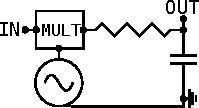
\includegraphics[width=4.5cm]{imgs/demodulador.pdf}
        \caption{Circuito demodulador}
    \end{center}
\end{figure}


Os circuitos foram implementados na especificação de simulação de circuitos/sinais mistos \texttt{NGSPICE}.

A figura seguinte demonstra as funcionalidades dos circuitos de modulação e demodulação, mostrando os resultados para as quatro combinações possíveis das duas entradas digitais ($S_{neutro}$ e $S_{alto}$). Foram usados um resistor de 1.5$\Omega$ e um capacitor de 100mF.

\begin{figure}[H]
    \begin{center}
        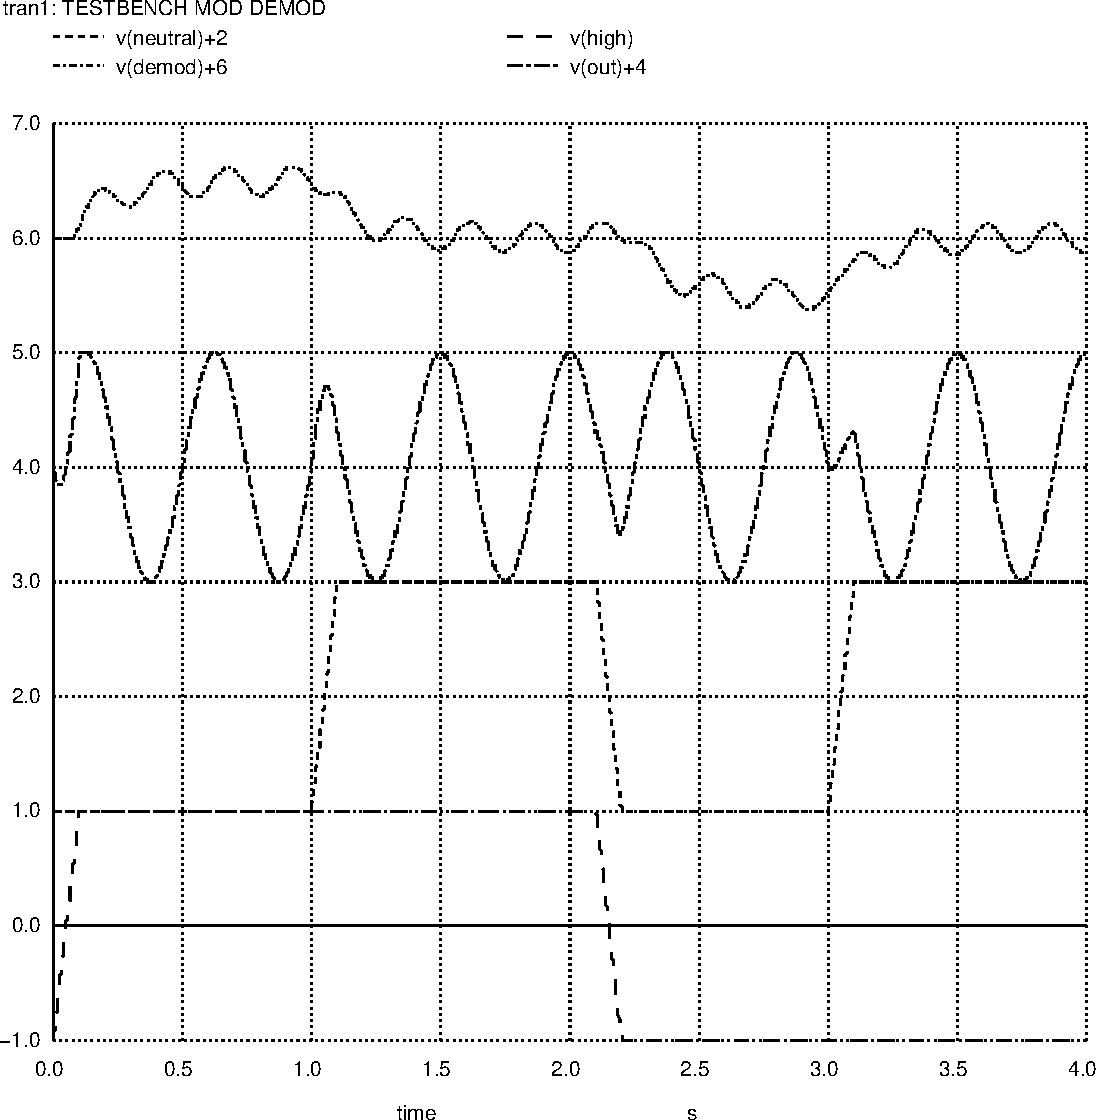
\includegraphics[width=9.5cm]{imgs/modemod.pdf}
        \footnotesize
        Em ordem:
        \begin{itemize}
            \item Sinal demodulado
            \item Sinal modulado
            \item $S_{neutro}$
            \item $S_{alto}$
        \end{itemize}
        \normalsize
        \caption{Resultado da simulação física}
    \end{center}
\end{figure}

Para a análise espectral, foi simulada uma sequência de 10 segundos de bits alternando-se entre 0 e 1 e aplicada a transformada rápida de Fourier nos sinais resultantes.

\begin{figure}[H]
    \begin{center}
        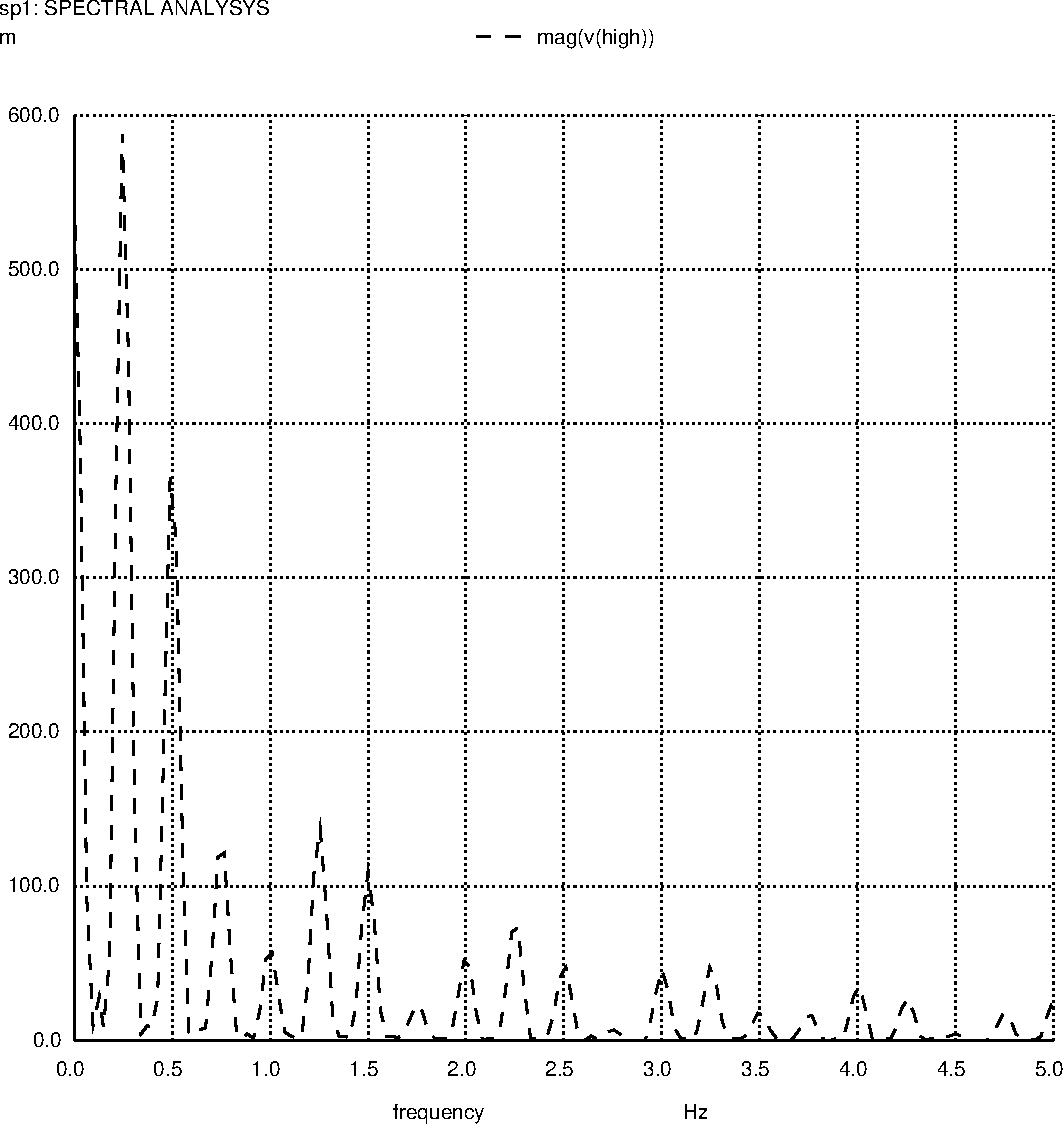
\includegraphics[width=7cm]{imgs/fftsquare.pdf}
        \caption{Análise espectral para o NRZ (sinal "high")}
    \end{center}
\end{figure}

Para a codificação NRZ (equivalente ao nosso sinal "high" no modulador), percebemos a esperada curva com os harmônicos baixos (e a constante - f=0) contribuindo com quase toda a energia do sinal.

\begin{figure}[H]
    \begin{center}
        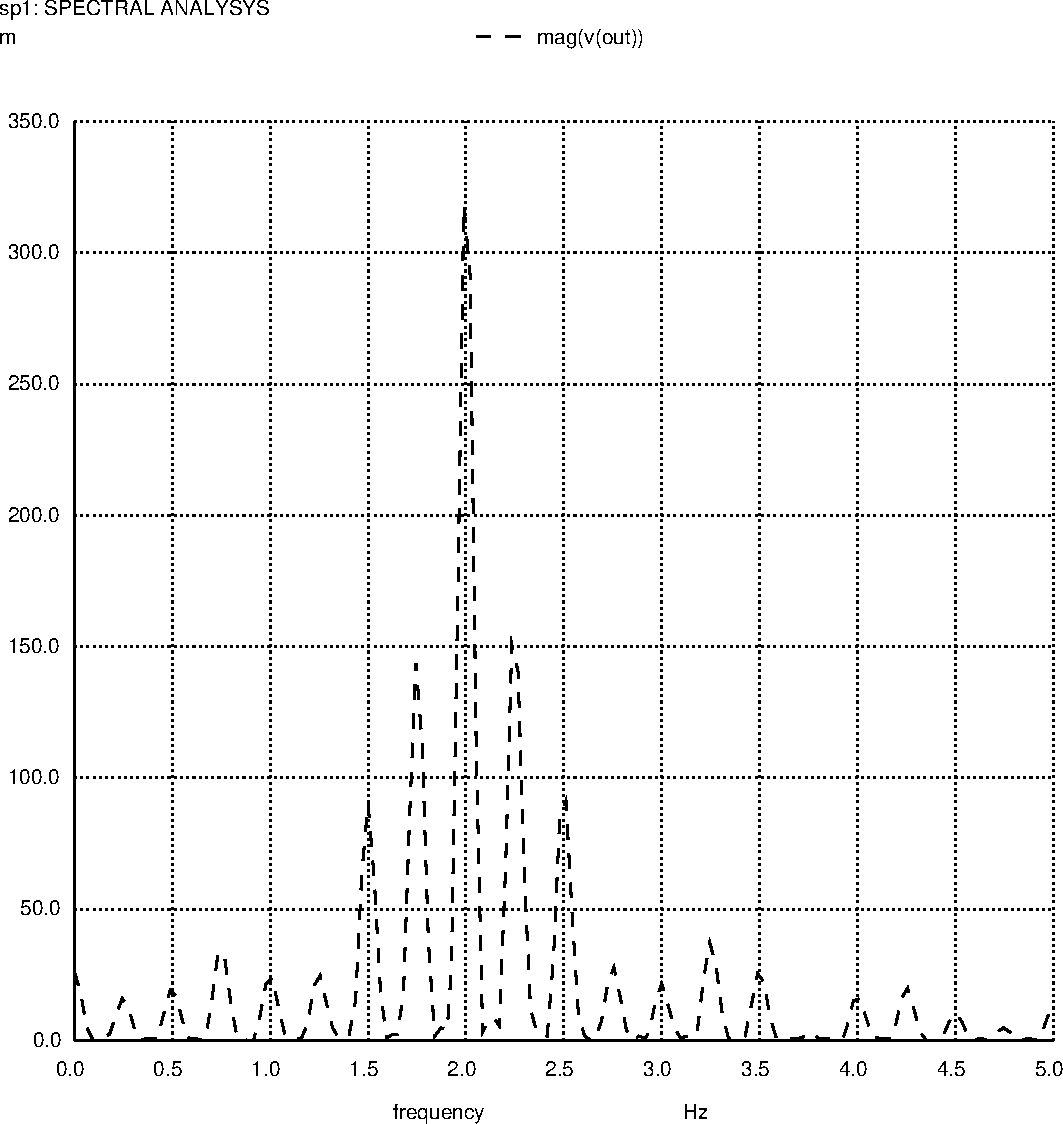
\includegraphics[width=7cm]{imgs/fftsig.pdf}
        \caption{Análise espectral para o sinal modulado}
    \end{center}
\end{figure}

Com a modulação, as componentes que carregam a maior energia se concentram ao redor da frequência da onda por\-ta\-do\-ra, garantindo que a energia está sendo usada na maior parte apenas para a transmissão de informações, além de permitir que sintonizemos o nosso receptor automaticamente ao buscar o pico principal.

\small
\begin{center}
    Todo o código aqui utilizado - inclusive o fonte deste relatório - está disponível no repositório \textit{https://github.com/m3101/TR1-P2}, que será aberto ao público ao final do prazo do projeto
\end{center}

\end{document}